\documentclass{article}

\usepackage{amsmath}
\usepackage{graphicx}
\usepackage{listings}
\usepackage{color}


\usepackage{xepersian}
\settextfont{BNazanin} 
\linespread{1.3}
\newcommand{\linia}{\rule{\linewidth}{0.5pt}}

\def\LOGO{
\begin{picture}(0,0)\unitlength=1cm
\put (0.5,0) {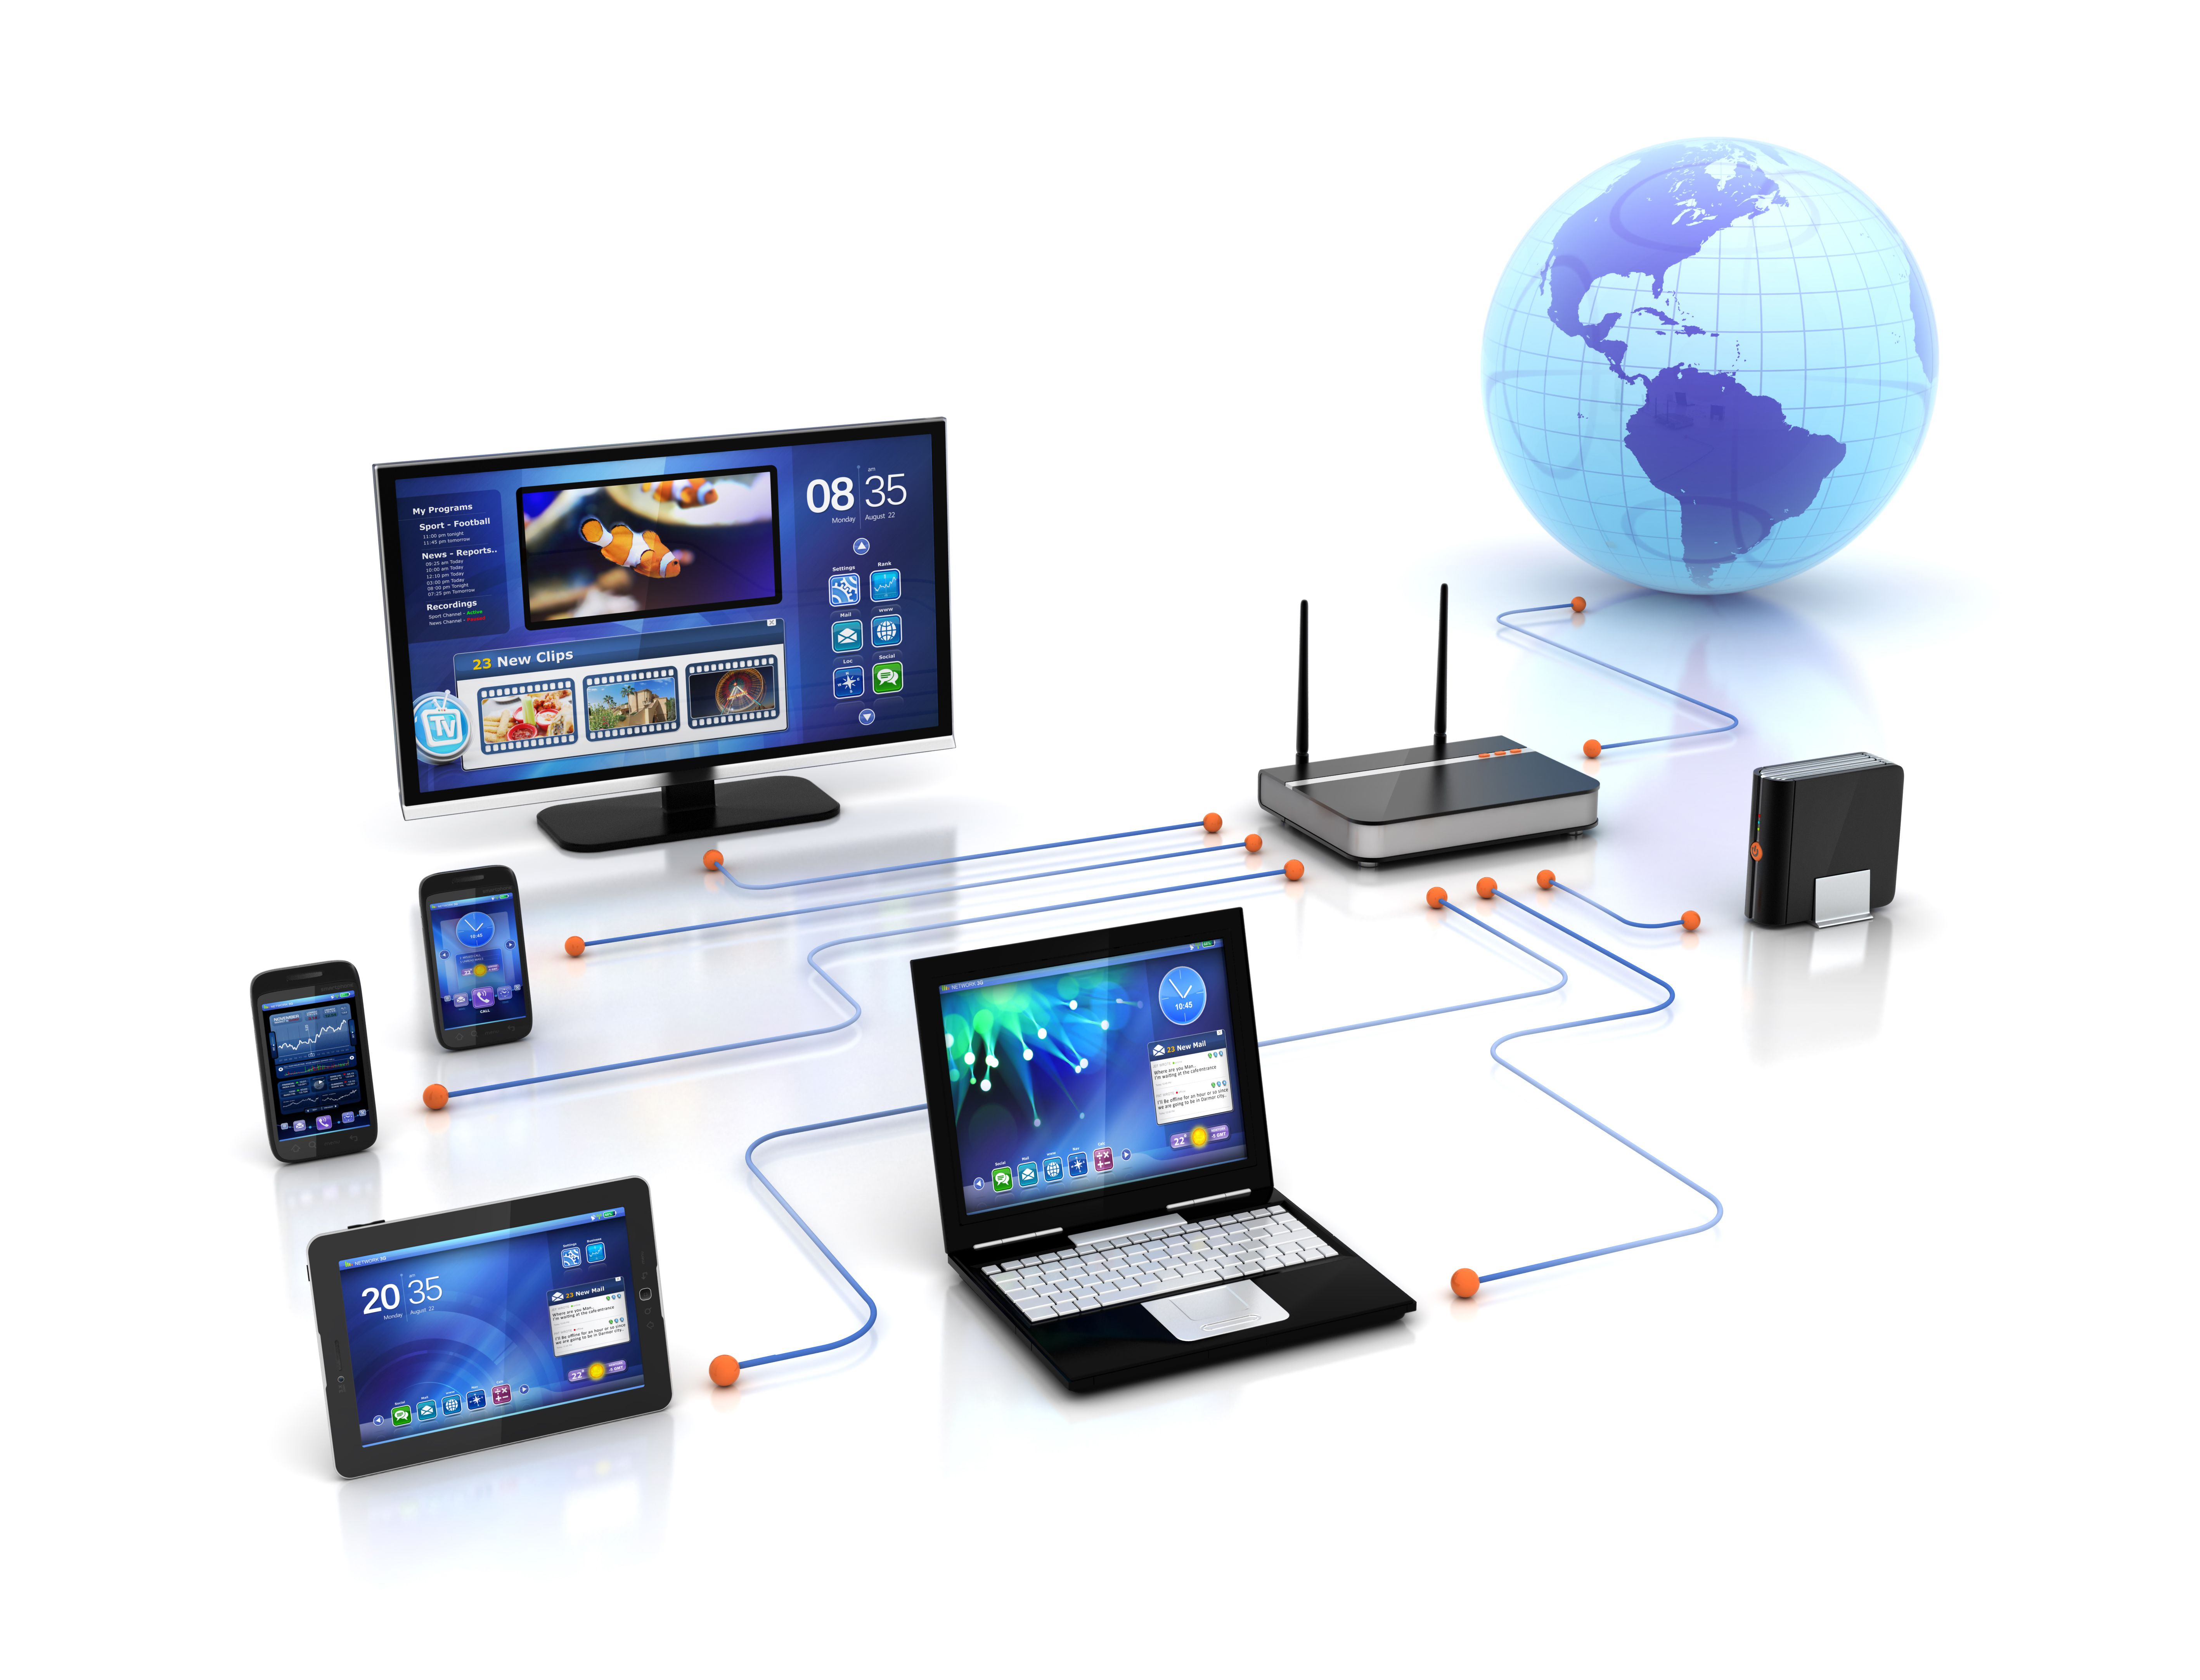
\includegraphics[width=5.1em]{network.jpg}}
\end{picture}
}

\def\LOG{
\begin{picture}(0,0)\unitlength=0.5cm
\put (-6,0) {
\includegraphics[width=4em]{question.png}}
\end{picture}
}

\definecolor{mygreen}{rgb}{0,0.6,0}
\definecolor{mygray}{rgb}{0.5,0.5,0.5}
\definecolor{mymauve}{rgb}{0.58,0,0.82}

\lstset{ 
  backgroundcolor=\color{white},   % choose the background color
  basicstyle=\footnotesize,        % size of fonts used for the code
  breaklines=true,                 % automatic line breaking only at whitespace
  captionpos=b,                    % sets the caption-position to bottom
  commentstyle=\color{mygreen},    % comment style
  keywordstyle=\color{blue},       % keyword style
  stringstyle=\color{mymauve},     % string literal style
}


\begin{document}

\title{\LOG        سوال ۳ کلاس استاد        \LOGO }
\author{نازنین صبری\\۸۱۰۱۹۴۳۴۶}
\date{ فروردین ۱۳۹۷}
\maketitle

\renewcommand{\labelenumii}{\alph{enumii}}
\begin{enumerate}
	\item  چگونه وب سرور چند کلاینت را روی یک پورت \lr{TCP} می‌پذیرد؟\\با توجه به مباحث تدریس شده در کلاس در اتصال به وب سرور برای هر درخواست متمایز یک اتصال جدید برقرار می‌کند و زمانی یک درخواست متمایز از سایرین است که ترکیب \lr{IP} و \lr{Port} آن متمایز باشد، مشابه شکل زیر.\\حال اگر از یک پردازه واحد (یعنی از یک \lr{IP} و \lr{Port} واحد) بخواهیم ۲ درخواست به یک وب سرور بفرستیم خود سیستم عامل به جای عدد پورت هر یک از این درخواست‌ها یک عدد رندوم قرار می‌دهد و پورت این درخواست را به این عدد رندوم \lr{map} می‌کند با این کار از نظر وب سرور شرایط تفاوتی با حالت قبل نکرده است و ۲ درخواست تمایز اند و انگار از ۲ پردازه مختلف آمده اند و این \lr{OS} است که این مسئله را هندل می‌کند و پس از آمدن پاسخ با استفاده از \lr{mapping} موجود پاسخ را به دست پردازه‌ی مورد نظر می‌رساند.\\ 
	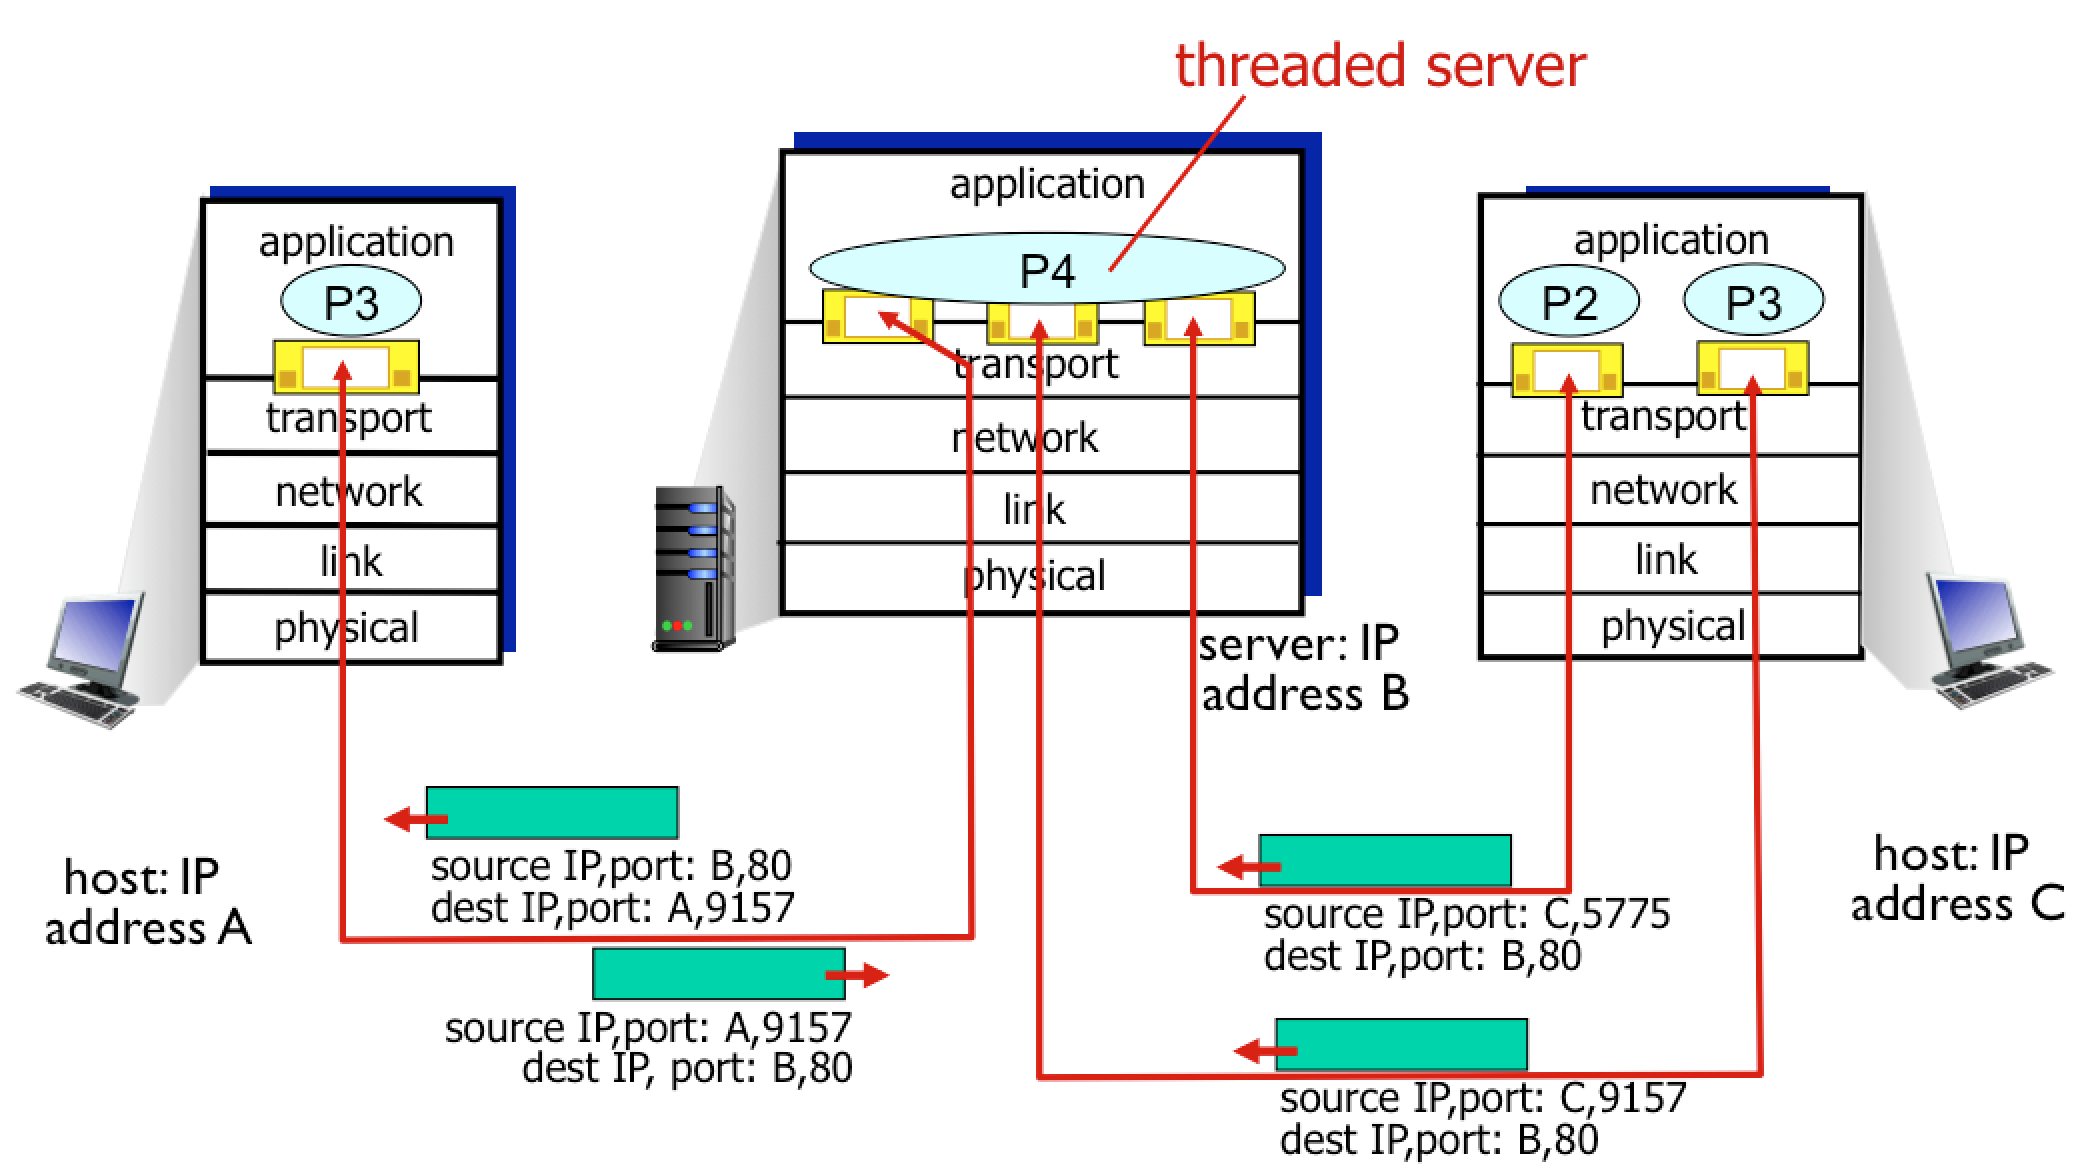
\includegraphics[scale=0.3]{./2Rec} 
\end{enumerate}


\end{document}